\documentclass{article}
\usepackage{amsmath}
\usepackage[francais]{babel}
\usepackage{amsfonts}
\usepackage{amssymb}
\usepackage[utf8]{inputenc}
\usepackage{graphicx}
\usepackage{color}
\usepackage[T1]{fontenc}
\usepackage{subfigure}

\begin{document}

\begin{section}{H.264}
La norme de compression vidéo H.264, aussi connu sous le nom de \textit{MPEG-4 
Part 10}, suscite un grand intérêt autant commercial qu'académique, vu ses
performances impressionnantes en regards des standards préexistants et les
technologies de pointe qui le composent. Ce standard, approuvé en mai 2003,
raffine les technologies de ces prédécesseurs MPEG-2 et H.263. De plus, il
intègre plusieurs innovations avant-gardistes. À ce jour, H.264 est un
incontournable pour les applications vidéos telles le \textit{Blu-Ray},
la télévision sur IP (\textit{IPTV}) et la lecture vidéo en transit ( \textit{streaming})
. Ce chapitre présente sommairement les concepts importants de la 
H.264 ainsi que les concepts liés à l'encodage vidéo.

\begin{subsection}{Survol}
Le standard H.264 offre, pour une fidélité visuelle comparable à MPEG-2, une économie 
de 50\% du débit \cite{sullivan2005}. Cette réalisation n'est pas l'œuvre d'une
innovation majeure, mais bien de l'effet combiné de plusieurs innovations dans
divers aspects de l'encodage vidéo. Pour mieux comprendre cette technologie,
commençons décrire sommairement les étapes d'encodage vidéo.

\begin{figure}[htb]
\centering
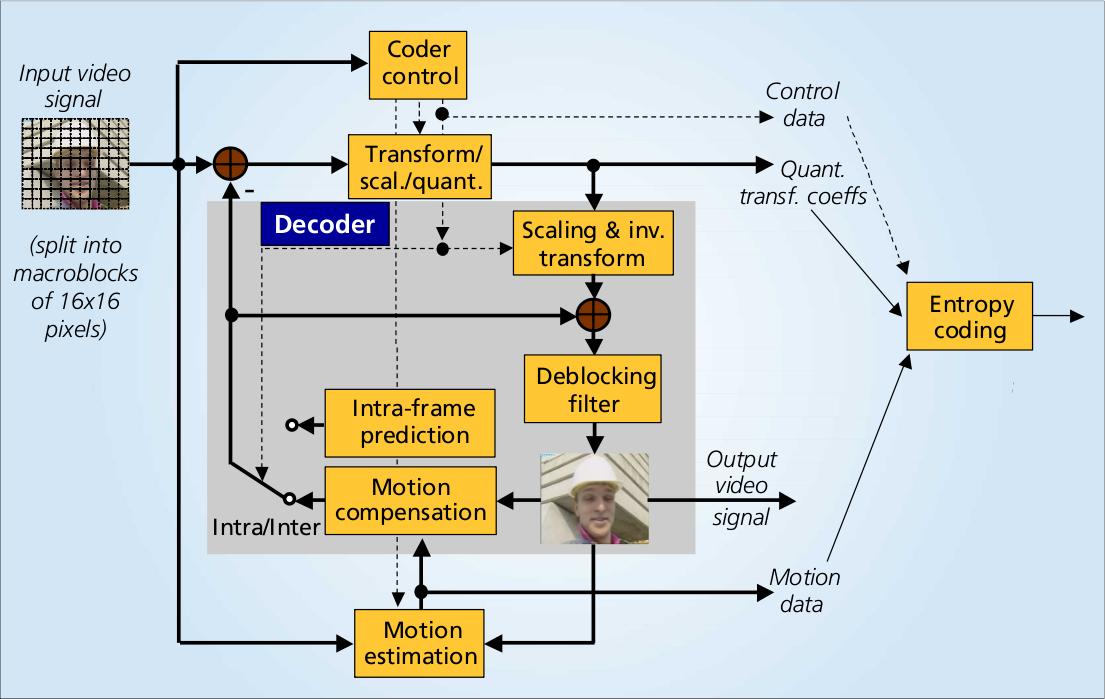
\includegraphics[width=\linewidth]{images/encoderOverview.png}
\caption{Survol des composantes de la norme H.264 ref. \cite{schafer2003}.}
\label{fig-EncoderOverview}
\end{figure}
(SC- il faut refaire tes figures en français, le faire plus tard)
(LT- modifier les blocs pour concorder avec le texte, le faire plus tard)

Tout d'abord, le signal vidéo est divisé en macroblocs. Ceux-ci démontrent une
forte corrélation spatiotemporelle, ce qui rend possible la prédiction de
macroblocs. La prédiction permet de réduire considérablement la quantité de données à
transmettre, il ne suffit qu'à transmettre les modes de prédiction utilisés ainsi que le
différentiel entre le bloc prédit et le bloc à encoder. La norme H.264 permet
deux types de prédiction. La première est basée sur les blocs d'une autre trame et appellée prédiction
(\textit{inter}). La seconde est obtenue en interpolant le contenu des blocs voisins et est appelée prédiction 
(\textit{intra}). Afin d'optimiser l'encodage entropique du différentiel,
celui-ci subit une transformée entière ainsi qu'une quantification. La division
du signal vidéo en macroblocs crée des effets de bloc dans l'image, ceux-ci sont
mitigés à l'aide du \textit{deblocking filter}.
\end{subsection}

\begin{subsection}{La prédiction de macrobloc}
\begin{subsubsection}{La prédiction de macrobloc \textit{inter}}
\newcommand{\ltMIN}[1]{\arg \min_{#1}}
\newcommand{\ltSAD}[1]{\textrm{SAD}(#1)}
\newcommand{\ltC}[1]{\mathbf{C}_{#1}}
\newcommand{\ltR}[1]{\mathbf{R}_{#1}}
Une source importante de redondance exploitée par la norme H.264 est la
redondance inter-image, souvent appelée \textit{inter}. La prédiction
\textit{inter} crée un modèle de prédiction basé sur une ou plusieurs trames
vidéo préalablement décodées \cite{richardson2003}. Ce modèle de prédiction est
fondé sur la recherche et la compensation de mouvement. (SC- selon moi c'est basé sur de l'appariement de blocs entre deux trames, i.e. trouver le bloc qui ressemble le plus à celui que l'on veut transmettre.)

\begin{figure}[htb]
\centering
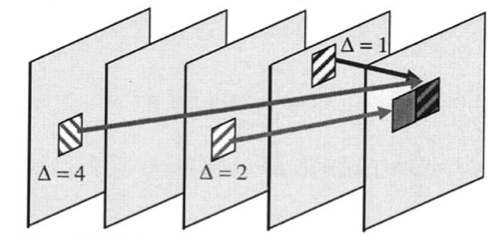
\includegraphics[scale=0.5]{images/multipicture.png}
\caption{Vecteurs de mouvements provenant de quatre trames vidéo préalablement
décodées, utilisées pour encoder un bloc dans la trame courante 
\cite{schafer2003}.}
\label{fig-MultiPicture}
\end{figure}

Tout d'abord, définissons un bloc comme un ensemble contigu de pixels de taille
$M \times N$. En H.264, les blocs peuvent être de taille 16x16, 8x8, 16x8, 8x16, 4x4, 8x4 et 4x8. Au lieu d'encoder directement les pixels d'un bloc, la prédiction
\textit{inter} vise, par la recherche de mouvements, à déterminer le bloc,
provenant d'une trame déjà décodée, le plus fidèle au bloc à encoder. Ceci mènera à une petite erreur de prédiction et donc à moins de bits à transmettre que .... (SC- il faut expliquer pourquoi une plus petite erreur de prédiction mène à une petite erreur résiduelle transmise et moins de bits. Mais je vois que ton prochain paragraphe revient sur la figure et ensuite on revient au problème du résiduel. Essait d'amener le lecteur à comprendre en définissant étape par étape les notions sans parler de choses futures qu'il ne peut pas comprendre pour l'instant.)

Tel qu'illustré à la Figure~\ref{fig-EncoderOverview}, l'encodeur décode 
les trames qu'il encode (SC- il décode ce qu'il encode, ça va surprendre le lecteur. Faut le dire autrement). Les trames décodées servent à améliorer la précision 
des prédictions, car elles tiennent compte des artefacts dus à l'encodage. Ceci
explique pourquoi la recherche de vecteurs de mouvements est effectuée dans les
trames préalablement décodées. (SC- je suis pas d'accord. aussi le lecteur aura de la difficulté à comprendre)

(SC- il faut commencer par définir les blocs à encoder et un bloc de la trame de référence situé à (u,v). etc. aussi SAD doit dépendre de C et R pas juste u et v, c'est quoi p?)

Soit $(u,v)$ le vecteur de mouvement entre le bloc à encoder et le bloc le plus
fidèle obtenu avec 
\begin{equation}
\label{eq-Vectors}
(u, v) = \ltMIN{(u,v) \in [-p, p] \times [-p, p]} \ltSAD{u, v}
\:,
\end{equation}
où la somme de la différence absolue (SAD) du bloc à la position $(x,y)$ 
dans la
trame courante $\ltC{}$ par rapport à une trame de référence $\ltR{}$ se
définit comme étant
\begin{equation}
\ltSAD{u,v} = \sum_{k=0}^{M-1}\sum_{l=0}^{N-1} \left| \ltC{x+k,y+l} -
\ltR{x+k+u,y+l+v} \right|\:.
\end{equation}

En supposant que le bloc à encoder et le bloc résultant de la recherche de
vecteurs de mouvements soient identiques, il ne suffirait que d'encoder
$(u,v)$ et le numéro de la trame de référence ($\Delta$) pour représenter le
bloc à encoder. Cependant, il en est rarement ainsi; il est souvent nécessaire
d'encoder le différentiel entre le bloc prédit et le bloc à encoder.

De plus, $(u,v)$ n'est  pas nécessairement composé d'entiers (le déplacement des objets ne se fait généralement pas par pas de pixels entiers). La norme H.264 permet
l'utilisation de vecteurs de mouvements pouvant être précis jusqu'au quart de pixel.
Deux approches d'interpolation distinctes sont utilisées pour le demi et le
quart de pixel. Le demi-pixel $\mathbf{b}$, dans la Figure~\ref{fig-HalfPel},
est obtenu à l'aide de l'équation suivante provenant de l'application d'un filtre à réponse impulsionnelle finie~:
\begin{equation}
\mathbf{b} = round \left(\frac{E - 5F + 20G + 20H - 5I + J}{32} \right)\:.
\end{equation}
Dans l'équation précédente, les positions des pixels E, F, G, H, I et J sont illustrées à la Figure~\ref{fig-HalfPel}.
\begin{figure}[htb]
\centering
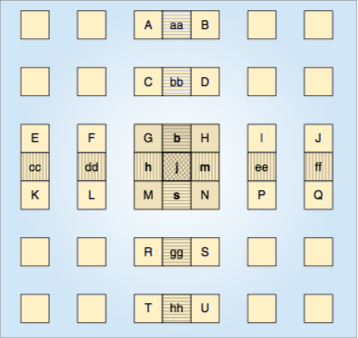
\includegraphics[scale=0.5]{images/HalfPel.png}
\caption{Interpolation au demi-pixel. Inspiré de \cite{richardson2003}.}
\label{fig-HalfPel}
\end{figure}

(SC- il faut présenter TOUTES les figures, ici on ne sais pas ce que sont E, F, . ce sont des valeurs de pixels à des positions entières, etc).
Pour les valeurs au quart de pixel, l'interpolation linéaire est utilisée entre les positions au demi pixel.
Soit $\mathbf{a}$ une valeur au quart de pixel située entre G et $\mathbf{b}$
dans la Figure~~\ref{fig-HalfPel}. On obtient $\mathbf{a}$ en effectuant
\begin{equation}
\mathbf{a} = round \left(\frac{G + \mathbf{b} }{2} \right)\:.
\end{equation}
Le filtre à réponse impulsionnelle finie de l'équation XX ainsi que l'interpolation linéaire précédente
sont utilisés seulement pour la luminance. Les
composantes chromatiques sont obtenues à l'aide d'une interpolation bilinéaire.
Pour obtenir la composante chromatique de $\mathbf{a}$, on a recourt à 
{\small\begin{equation}
\mathbf{a} = round \left( \frac{(8 - d_x) \cdot (8-d_y)A + d_x \cdot (8 - d_y)B
+ (8 - d_x) \cdot d_yC + d_x \cdot d_yD}{64} \right)\:.
\end{equation}} 
Où A, B, C, D sont les valeurs chromatiques des pixels entiers entourant la valeur à interpoler. Cette dernière est située à une distance $(d_x,d_y)$ de (SC- QUOI exactement? Pas clair car on ne sait même pas comment A,B,C et D sont disposés dans faire du reverse engineering e la formule)

(Pourquoi ne pas commencer par présenter cela dans ta section? Il faut vraiment présenter les choses dans un ordre logique pour quelqu'un qui connais pas ou peu la video)
Cela dit, un macrobloc contient $16 \times 16$ valeurs de luminances qui
peuvent être décomposés de quatre manières distinctes~: une partition $16 \times 16$,
deux partitions $16 \times 8$, deux partitions $8 \times 16$ et quatre
partitions $8 \times 8$. De plus, chacun des sous-macroblocs $8 \times 8$ peut
également être décomposé~: deux partitions $8 \times 4$, deux partitions $4 
\times
8$, et quatre partitions  $4 \times 4$. Le tout est résumé à la
Figure~\ref{fig-MacroblockPartitions}.

\begin{figure}[htb]
\centering
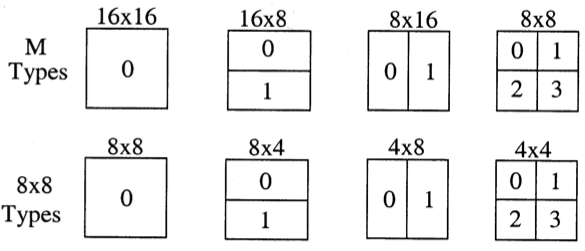
\includegraphics[scale=0.5]{images/MacroblockPartitions.png}
\caption{Partitions de macrocblocs et de sous-macroblocs
\cite{schafer2003}.}
\label{fig-MacroblockPartitions}
\end{figure}
(SC- il me semble que tu dois mettre la référence dans la figure sans mettre ref.)

La séparation de macroblocs permet d'optimiser l'encodage selon le niveau de
détails d'une surface. Un macrobloc $16 \times 16$ est efficace pour les 
régions lisses avec peu d'énergie. (SC-faux, ça peut être efficace pour une grande zône avec mouvement uniforme et translationnel)

Des partitions plus petites sont utiles
lorsque le différentiel entre la prédiction et le bloc à encoder est élevé (SC- revoir, c'est pour un bloc ne suivant pas mvmt uniforme ou translationnel).
Elles permettent d'utiliser plusieurs vecteurs de mouvements (un par partition)
pour mieux modéliser la surface. Cependant, les vecteurs de mouvements 
supplémentaires doivent, eux aussi, être transmis; ce qui décourage l'usage inutile de petites partitions.

Lorsque le nombre de partitions est élevé, encoder les vecteurs de mouvements 
de chacune d'elles peut engendrer un coût binaire considérable et particulèrement à bas débit. C'est
pourquoi, dans la norme H.264, les vecteurs de mouvements sont encodés
différentiellement à l'aide de la médiane ou d'une prédiction directionnelle
guidée par les blocs voisins \cite{wiegand2003}. Cette prédiction est 
efficace, car la redondance inter-trame cause une forte corrélation entre les
vecteurs de mouvements de blocs avoisinants. Les blocs utilisés pour la
prédiction sont des blocs préalablement décodés, qui appartiennent à la même
tranche que le bloc à prédire.
\end{subsubsection}

\begin{subsubsection}{La prédiction de macrobloc \textit{intra}}
Une seconde source considérable de redondance exploitée par la norme H.264 est
la redondance spatiale à l'intérieur d'une image, aussi connue sous le nom de
\textit{intra} (SC- la redondance ne porte pas le nom de intra). La prédiction \textit{intra} vise à modéliser la texture d'un
bloc à partir celle des blocs avoisinants.

À l'égal de l'encodage \textit{inter}, l'encodage \textit{intra} repose sur le
concept de blocs et de macroblocs (SC-tu n'as pas défini formellement c'est quoi un bloc et un macrobloc). On y retrouve également la notion de
blocs à tailles variables visant à optimiser l'encodage en fonction de la
variation du niveau d'énergie d'une surface (SC- variation du niveau d'énergie d'une surface?) . La norme H.264 permet à l'encodeur
de choisir entre des macroblocs $16 \times 16$ ou des sous-blocs $4 \times 4$ (SC- luma?).
Selon le choix, différents modes de prédiction sont offerts.

Fait intéressant, la prédiction \textit{intra} étant accomplie dans le domaine
spatial (contrairement à H.263 et MPEG-4 Visual qui utilisent le domaine
fréquentiel (SC mettre ref)). Toutefois, une telle pratique peut mener à une propagation
d'erreurs, si la prédiction repose sur des données corrompues. (SC- comment est-ce différent que ce soit dans le domaine spatial ou fréquentiel?)

L'approche prédictive réduit considérablement la quantité de données à 
encoder (SC- redondance). En outre, seulement le mode de prédiction et le différentiel entre le
bloc à encoder et le bloc prédit doivent être transmis. Quoique le différentiel 
comporte le même nombre de pixels, l'énergie de ceux-ci est moindre, ce qui en
facilite (SC- pas plus facile, juste plus efficace) l'encodage dans les étapes subséquentes.

La norme H.264 définit 9 modes de prédiction liés à l'utilisation de blocs 
$ 4 \times 4$. Huit de ces modes sont des extrapolations directionnelles à des
angles de 26.6$^\circ$, 45$^\circ$ et 90$^\circ$, tandis que le mode~2, aussi
connu sous le sigle DC, est la moyenne des pixels A à D et I à J (voir
Figure~\ref{fig-4x4PredictionModes}) préalablement encodés.

\begin{figure}[htb]
\centering
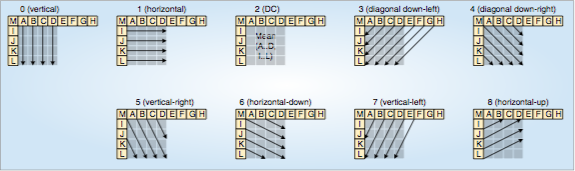
\includegraphics[width=\linewidth]{images/4x4PredictionModes.png}
\caption{Les modes prédictifs pour la luminance de blocs $4 \times 4$, inspiré
de \cite{richardson2003}.}
\label{fig-4x4PredictionModes}
\end{figure}
(SC fontes trop petites dans la figure, la faire sur 4 lignes)

Soit $\mathbf{d}$, le pixel situé dans le coin supérieur droit du bloc $4 
\times 4$ prédit par le mode~4 (diagonale sud-est). On obtient $\mathbf{d}$ à
l'aide de la formule suivante~:

\begin{equation}
\mathbf{d} = round \left(\frac{B + 2C + D}{4} \right)\:.
\end{equation}

La Figure~\ref{fig-4x4PredictionBlocks} illustre la prédiction obtenue pour
chaque mode offert pour un bloc $4 \times 4$ ainsi que la somme de l'erreur
absolue (SAE) obtenue entre la prédiction et le bloc à encoder. Dans cet exemple, le
meilleur mode de prédiction serait 8, car il offre le plus petit SAE, soit 203.

\begin{figure}%[htb]
\centering
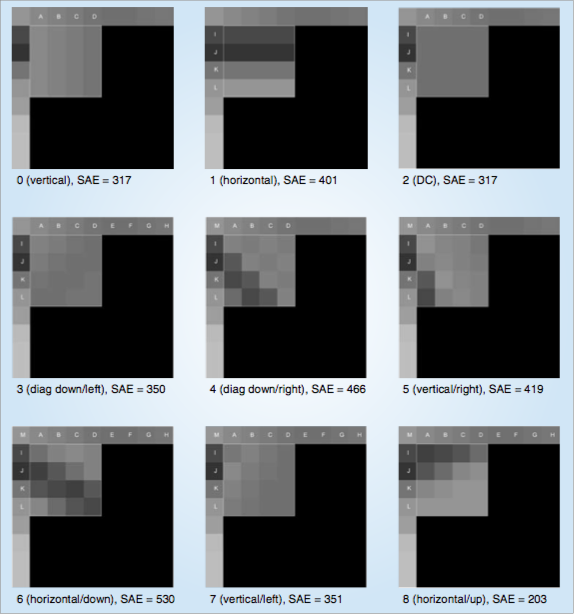
\includegraphics[width=\linewidth]{images/4x4PredictionBlocks.png}
\caption{Résultats de la prédiction des différents modes de blocs $4 \times 4$,
inspiré de \cite{richardson2003}.}
\label{fig-4x4PredictionBlocks}
\end{figure}
(SC- il est unitile de montrer le SAE si on ne voir pas le bloc à encoder)

Tel qu'illustré à la (SC- figure en minuscule dans un texte français, partout sauf les figures elles-mêmes) Figure~\ref{fig-16x16PredictionModes}, H.264 spécifie quatre
modes de prédiction de macroblocs $16 \times 16$~: horizontal, vertical, DC et
plane. DC utilise la moyenne des pixels limitrophes horizontaux et verticaux,
tandis que les trois autres approches sont des extrapolations. Contrairement aux
$4 \times 4$, les modes de prédictions $16 \times 16$ sont destinés aux surfaces
lisses avec peu de variation d'énergie, ceci explique pourquoi ceux-ci sont plus
simples.

\begin{figure}%[htb]
\centering
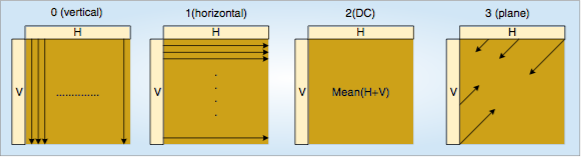
\includegraphics[width=\linewidth]{images/16x16PredictionModes.png}
\caption{Modes de prédiction de la luminance de blocs $16 \times 16$, inspiré
de \cite{richardson2003}.}
\label{fig-16x16PredictionModes}
\end{figure}
(SC-fontes trop petites)

En ce qui concerne les composantes chromatiques, celles-ci se regroupent dans un
bloc $8 \times 8$, vu le sous-échantillonnage chromatique (SC-pas expliqué). Les mêmes types de
prédictions que pour les blocs $16 \times 16$ sont employés soient~: DC,
horizontal, vertical et plane. Ceci est lié au fait que dans les
images naturelles, les composantes chromatiques varient beaucoup moins que la
luminance; ceci en facilite la prédiction.

La norme H.264 inclut un mode I\_PCM. Ce mode, souvent réservé aux blocs
anormaux, se distingue par l'absence de prédiction et de transformée. Dans
certains contextes, ce mode peut être plus avantageux que l'utilisation d'une
prédiction. Par exemple, le cas ou un bloc distinct nuirait aux prédictions
subséquentes. Dans un tel cas, I\_PCM permet à l'encodeur d'éviter 
l'altération de la prédiction, ce qui peut être moins couteux à long terme que
d'encoder le bloc distinct sans prédiction. (SC-pourquoi en parler si ton projet ne l'utilise pas?)
\end{subsubsection}
\end{subsection}


\begin{subsection}{La transformée}
\newcommand{\ltH}{\mathbf{H}}
Les approches présentées jusqu'à présent cherchent à éliminer la redondance
spatiotemporelle d'une sequence vidéo par l'utilisation de prédictions. Ces
prédictions reposent sur les corrélations intrisèques aux données d'une séquence
vidéo. Ces prédictions sont imparfaites et requièrent que le différentiel entre la
prédiction et le bloc à encoder soit, lui aussi, encodé. Toutefois, ce
différentiel, appelé erreur résiduelle, possède une forte autocorrélation. La transformée entière
définie dans la norme H.264, a pour objectif de décoréler le différentiel afin
d'en faciliter l'encodage. La matrice de transformation
\begin{equation}
\ltH = \begin {bmatrix}
1 & 1 & 1 & 1\\
2 & 1 & -1 & -2\\
1 & -1 & -1 & 1\\
1 & -2 & 2 & -1
\end{bmatrix}
\end{equation}
possède des propriétés similaires à une transformée en cosinus discrète 
(DCT) $4 \times 4$ \cite{malvar2003}, qui est très prisée pour son aptitude
à décorreller un ensemble de données.

La transformée entière possède plusieurs avantages par rapport à la DCT.
D'une part, elle est plus simple et requiert seulement des additions et
des décallages binaires (\textit{bit shift}). D'autre part, son résultat étant
entier, il n'y a pas de perte fractionnaires lors de la transformée inverse.

H.264 applique sa transformée sur des blocs $4 \times 4$, ceci la distingue de
ses prédécesseurs qui utilisent des blocs $8 \times 8$. L'utilisation de blocs
plus petits est justifiée par les améliorations substantielle de la  précision
des prédictions \textit{intra} et \textit{inter}, qui réduisent considérablement
le résiduel à transformer. De plus, l'utilisation de blocs plus petits réduit grandement
le bruit autour des bordures (souvent appellé \textit{ringing} ou
\textit{musquito noise}). L'ordre de balayage des différentiels de blocs $4
\times 4$ est présenté à la Figure~\ref{fig-Transform}.

\begin{figure}[htb]
\centering
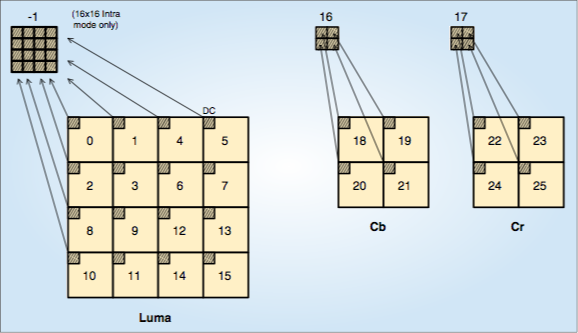
\includegraphics[width=\linewidth]{images/Transform.png}
\caption{Ordre de balayage des coefficients de blocs à
l'intérieur d'un macrobloc lors d'une transformée entière $4 \times 4$. \cite{richardson2003}.}
\label{fig-Transform}
\end{figure}

\end{subsection}

\begin{subsection}{La quantification}
Une nouveauté de la norme H.264, est qu'elle définit un paramètre de
quantification qui exerce un contrôle logarithmique sur le pas de
quantification, ses prédécesseurs utilisaient un contrôle linéaire. Le
quantificateur est scalaire et peut varier pour la luminance et les composantes
chromatiques. La valeur quantifiée $Z$ de la valeur transformée $Y$ à la
position $i,j$ est définit comme étant :
\begin{equation}
Z_{ij} = round\left(\frac{Y_{ij}}{Qstep}\right)
\end{equation}
Où $Qstep$ est le pas de quantification et $round$ la fonction d'arrondissement
afin d'obtenir des résultats entiers. La norme définit 52 valeurs de pas de
quantification indexées par le paramètre de quantification (QP), une
augmentation de 6 de ce dernier double le pas de quantification. Ce grand nombre
de valeurs permet à l'encodeur une meilleure précision, en ce qui a trait au
compromis entre le débit binaire et la qualité visuelle.
\end{subsection}

\begin{subsection}{L'encodage entropique}
La norme H.264 innove dans le domaine du codage entropique en séparant le codage
des paramètres de celui des données. Pour l'encodage de paramètres, ceux-ci sont
représentés par des codes numériques qui sont encodés avec des codes à longueur
variable appelés codes exponentiel-Golomb. Les valeurs des différentiels de
prédiction sont encodées soit avec un codage entropique à longueur variable
(CAVLC) ou un codage arithmétique binaire à contexte adaptatif (CABAC). Bien que
CABAC offre de gain de compression d'environ 10\% par rapport à CAVLC, ce
dernier est prédominant dans les applications mobiles vu sa simplicité. C'est
pour cette raison que dans cet ouvrage, nous concentrons nos efforts
exclusivement sur la CAVLC.

\begin{subsubsection}{Le codage exponentiel-Golomb} (SC- est-ce que cette section est utile. elle me semble trop détaillée pour nos besoins et pas assez pour comprendre. Quel est le but de mettre cela?)
L'encodage à taille variable exponentiel-Golomb est fortement structuré et
se résume par~:
\begin{equation}
[M~\text{zéros}]1[\text{suffixe}]
\end{equation}
Ce code se divise en trois parties~: préfixe, 1 et suffixe. Le préfixe
est composé de $M$ zéros. Par la suite, un 1 est ajouté dénotant la fin du
préfixe. Finalement, le suffixe, de longueur $M$, contient le code numérique
sous format binaire.

Soit $c$, un entier représentant un code numérique. Le nombre de zéros contenus
dans son préfixe est défini par
\begin{equation}
M = \lfloor \log_2(c+1) \rfloor \:,
\end{equation}
et son suffixe est obtenu à l'aide de 
\begin{equation}
\text{suffixe} = c + 1 - 2^M \:.
\end{equation}
\end{subsubsection}

\begin{subsubsection}{CAVLC} (SC-me semble incomplet. un exemple à moitié complété, des explications théoriques incomplètes, on pourrait mentionner les aspects importants comme un bit en erreur brise beaucoup l'information, perd la sync, etc.)
L'encodage entropique à contexte adaptatif (CAVLC) est un encodage qui utilise
une table de référence et qui est optimisée pour encoder les différentiels de
prédictions transformés, quantifiés. Les différentiels à encoder possèdent des caractéristiques
très intéressantes~: ils se terminent par un grand nombre de zéros, on y
retrouve des 1 dispersés et les données sont concentrées autour du coin
supérieur gauche.

Voici l'exemple d'un bloc $4 \times 4$ provenant du différentiel de la
prédiction et du bloc décodé, qui par la suite, a été transformé et quantifié.
\begin{equation*}
\begin {bmatrix}
8 & 3 & 1 & 0\\
7 & 0 & 0 & 0\\
1 & 0 & 0 & 0\\
0 & 0 & 0 & 0
\end{bmatrix}
\end{equation*}
Ce bloc est lu en ordre \textit{Zig-Zag}, ce qui donne la suite suivante de
chiffres~:
\begin{equation*}
8,~3,~7,~1,~0,~1,~0,~0,~0,~0,~0,~0,~0,~0,~0,~0,~0 
\end{equation*}
Pour encoder ces chiffres avec CAVLC, on commence par encoder les valeurs
supérieures à 1 en ordre \textit{Zig-Zag} inversé (7,3 et 8) à l'aide d'une
table de référence. Pour les 1 et 0 constituant la fin de la série, quatre
paramètres, décrits à la table~\ref{tab-CAVLC}, sont utilisés.

\begin{table}[htb]
\caption{Paramètres qui régissent l'encodage de la série de 1 et 0 qui terminent
un différentiel de prédiction transformé, quantifié}.
\label{tab-CAVLC}
\vspace{1em}
\centering
\small
\begin{tabular}{ l p{2,5cm} p{7cm} }
 \hline
 Paramètre & Valeur (\textit{pour~exemple}) & Description  \\
 \hline
$N$ & 5 &Le nombre de valeurs supérieures à 0.\\
$T1$ & 2 &Le nombre de 1.\\
$TZ$ & 1 &Le nombre de 0, commençant du début de la séquence jusqu'à la dernière
valeur supérieure à 0.\\
$RB$ & 1 &Le nombre de 0 entre les deux dernières valeurs supérieures à 0.\\
\hline   
\end{tabular}
\end{table}

\end{subsubsection}

\end{subsection}

\begin{subsection}{Le \textit{deblocking filter}}
Le filtre anti-blocs, mieux connu sous son nom anglophone \textit{deblocking
filter}, a pour objectif de réduire l'apparence d'effets de bloc (variation
importante de la valeur des pixels en bordure de blocs). L'effet secondaire le
plus important produit par les algorithmes de compression vidéo présents dans la
norme H.264 (SC-pas de verbe dans la phrase?). Il est le produit d'une discontinuité spatiale provenant de
variations d'encodage de blocs adjacents.

\begin{figure}[htb]

\centering
\subfigure[Sans «~deblocking filter~»]{
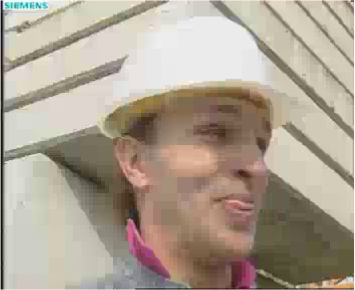
\includegraphics[width=0.47\linewidth]{images/ForemanWithoutDeblocking.png}
}
\subfigure[Avec «~deblocking filter~»]{
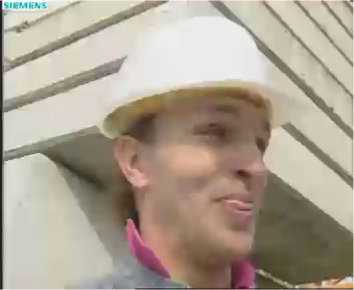
\includegraphics[width=0.47\linewidth]{images/ForemanWithDeblocking.png}
}
\caption{Performance du \textit{deblocking filter} pour une trame fortement
compressée ref. \cite{schafer2003}.}
\label{fig-Deblocking}
\end{figure}

Le \textit{deblocking filter} agit en bordure de blocs dans le but de lisser les
variations importantes d'intensités des valeurs de pixels, comme  qu'illustré
à la Figure~\ref{fig-Deblocking}. Beaucoup plus qu'un simple filtre, le
\textit{deblocking filter} (SC-French please) tient compte du pas de quantification ainsi que du
type de prédiction utilisé pour encoder les blocs, afin d'ajuster l'intensité
du lissage.

La norme H.264 definit deux seuils qui régissent le comportement du 
\textit{deblocking filter}. Soit $\alpha$ pour l'écart entre les pixels en
bordure de deux blocs~:
\begin{equation}
\left| p_0 - q_0 \right| < \alpha(Indice_A)  (SC-ne pas mettre indice en italic)
\end{equation}
et $\beta$ pour l'écart entre les pixels à la bordure d'un même bloc~:
\begin{align}
\left| p_1 - p_0 \right| < \beta(Indice_B)\\
\left| q_1 - q_0 \right| < \beta(Indice_B)\:.
\end{align}
\begin{figure}[htb]
\centering
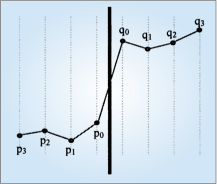
\includegraphics[scale=0.65]{images/BlockyEdge.png}
\caption{Visualisation unidimensionelle d'une bordure de bloc qui requiert
l'intervention du «~deblocking filter~», inspiré de \cite{list2003}.}
\label{fig-BlockyEdge}
\end{figure}
Où $p$ et $q$ sont les pixels en bordure de blocs tel qu'illustré à la
Figure~\ref{fig-BlockyEdge}, l'encodeur peut biaiser les $Indices$ à l'aide 
d'un
décalage tel que
\begin{align}
Indices_A(x) &= \min(\max(0,QP+Decalage_A), 51)\\ (SC-ne pas mettre décalage en italic)
Indices_B(x) &= \min(\max(0,QP+Decalage_B), 51)\:.
\end{align}
La plage de valeur de 0 à 51 représente les valeurs possibles du paramètre de
quantification ($QP$)(SC-qu avais utilisé QP au lieu de $QP$ avant faut être uniforme). Cela dit, dans la formule précédente QP est le paramètre
de quantification moyen entre les deux blocs évalués. Les valeurs des seuils
$\alpha$ et $\beta$ sont définies à l'aide des formules suivantes~:
\begin{align}
\alpha(x) &= 0.8(2^{x/6}-1)\\
\beta(x) &= 0.5x-7
\end{align}
(SC-définir x dans la formule précédente)

Afin de savoir si un lissage doit être appliqué, et si oui, à quelle
intensité, le paramètre d'intensité de la bordure (bS) est défini selon des
règles basé sur le mode d'encodage. Celles-ci sont résumées dans la table
\ref{tab-FilteringRules}.

\begin{table}[htb]
\caption{Règles guidant l'intensité du deblocking filter en fonction des
conditions d'encodages.}
\label{tab-FilteringRules}
\vspace{1em}
\centering
\begin{tabular}{ l l }
 \hline
 Condition d'encodage & Intensité \\
 \hline   
 Prédiction Intra et en bordure de macrobloc & 4 (Lissage fort)\\
 Prédiction Intra & 3 \\
 Prédiction Inter et présence de résiduel & 2 \\
 Différence des vecteurs de mouvement $\geqslant$ 1 & 1 \\
 Prédiction Inter avec des trames de références différentes& 1 \\
 Sinon & 0 (Aucun lissage) \\ 
 \hline   
\end{tabular}
\end{table}

Comme le démontre la table~\ref{tab-FilteringRules}, le type de
prédiction et les conditions d'encodage produisent différents degrés d'effet
de bloc. C'est pourquoi il est crucial que le filtre soit ajustable. De plus,
les seuils $\alpha$ et $\beta$ permettent de prendre en compte la texture propre
à l'image afin de ne pas lisser des variations de valeurs de pixels propres à
l'image situés en bordure de blocs.

L'usage du \textit{deblocking filter} permet, pour un même niveau de qualité (
mesuré avec le PSNR), d'obtenir une réduction du débit de 5 à 10\% selon le
contexte \cite{list2003}. Ce mécanisme est un ajout important de H.264 qui
le différencie de ces prédécesseurs. Quoique plusieurs utilisaient des
\textit{deblocking filter}, peu le rendaient obligatoire comme le fait la norme
H.264. Son ajout dans la chaîne d'encodage décodage fait en sorte que ses
améliorations sont prises en compte lors des prédictions inter-image.
\end{subsection}

\bibliographystyle{IEEEbib}
\bibliography{h264}
(SC- il y a h.264 avc dans la biblio, il faut H.264 et AVC)
\end{section}

\end{document}

